% Template Created by Albert Alises Sorribas (albert.alises@gmail.com) for the thesis of the MSc. in Computational Biomedical Engineering, Universitat Pompeu Fabra. Based on the thesis template of the Imperial College London,  downloadable at http://www.imperial.ac.uk/brand-style-guide/templates/downloadable-templates/

\documentclass[a4paper,12pt,twoside]{report}
\usepackage[left=3cm,right=3cm,top=3cm,bottom=3cm]{geometry} %Margins
\usepackage{pdfpages}
\usepackage{hyperref}
\usepackage{listings}
\usepackage{xcolor}
\usepackage{setspace}
\usepackage{tocloft}
\usepackage{amsmath}
\usepackage{chngcntr }
\usepackage[toc,page]{appendix}
\usepackage[T1]{fontenc}
\usepackage[nottoc]{tocbibind}
\usepackage[compact]{titlesec}
\titlespacing{\section}{0pt}{1ex}{0ex}
\titlespacing{\subsection}{0pt}{1ex}{0ex}
\titlespacing{\subsubsection}{0pt}{1ex}{0ex}

\counterwithout{figure}{chapter}
\counterwithout{table}{chapter}

\usepackage{graphicx}
\usepackage{verbatim}
\usepackage{latexsym}
\def\bbbr{{\rm I\!R}} %reelle Zahlen
\def\bbbm{{\rm I\!M}}
\def\bbbn{{\rm I\!N}} %natuerliche Zahlen
\def\bbbf{{\rm I\!F}}
\def\bbbh{{\rm I\!H}}
\def\bbbk{{\rm I\!K}}
\def\bbbp{{\rm I\!P}}
\def\bbbe{{\rm I\!E}}
\def\bbbone{{\mathchoice {\rm 1\mskip-4mu l} {\rm 1\mskip-4mu l}
{\rm 1\mskip-4.5mu l} {\rm 1\mskip-5mu l}}}
\def\bbbc{{\mathchoice {\setbox0=\hbox{$\displaystyle\rm C$}\hbox{\hbox
to0pt{\kern0.4\wd0\vrule height0.9\ht0\hss}\box0}}
{\setbox0=\hbox{$\textstyle\rm C$}\hbox{\hbox
to0pt{\kern0.4\wd0\vrule height0.9\ht0\hss}\box0}}
{\setbox0=\hbox{$\scriptstyle\rm C$}\hbox{\hbox
to0pt{\kern0.4\wd0\vrule height0.9\ht0\hss}\box0}}
{\setbox0=\hbox{$\scriptscriptstyle\rm C$}\hbox{\hbox
to0pt{\kern0.4\wd0\vrule height0.9\ht0\hss}\box0}}}}
\def\bbbq{{\mathchoice {\setbox0=\hbox{$\displaystyle\rm
Q$}\hbox{\raise
0.15\ht0\hbox to0pt{\kern0.4\wd0\vrule height0.8\ht0\hss}\box0}}
{\setbox0=\hbox{$\textstyle\rm Q$}\hbox{\raise
0.15\ht0\hbox to0pt{\kern0.4\wd0\vrule height0.8\ht0\hss}\box0}}
{\setbox0=\hbox{$\scriptstyle\rm Q$}\hbox{\raise
0.15\ht0\hbox to0pt{\kern0.4\wd0\vrule height0.7\ht0\hss}\box0}}
{\setbox0=\hbox{$\scriptscriptstyle\rm Q$}\hbox{\raise
0.15\ht0\hbox to0pt{\kern0.4\wd0\vrule height0.7\ht0\hss}\box0}}}}
\def\bbbt{{\mathchoice {\setbox0=\hbox{$\displaystyle\rm
T$}\hbox{\hbox to0pt{\kern0.3\wd0\vrule height0.9\ht0\hss}\box0}}
{\setbox0=\hbox{$\textstyle\rm T$}\hbox{\hbox
to0pt{\kern0.3\wd0\vrule height0.9\ht0\hss}\box0}}
{\setbox0=\hbox{$\scriptstyle\rm T$}\hbox{\hbox
to0pt{\kern0.3\wd0\vrule height0.9\ht0\hss}\box0}}
{\setbox0=\hbox{$\scriptscriptstyle\rm T$}\hbox{\hbox
to0pt{\kern0.3\wd0\vrule height0.9\ht0\hss}\box0}}}}
\def\bbbs{{\mathchoice
{\setbox0=\hbox{$\displaystyle     \rm S$}\hbox{\raise0.5\ht0\hbox
to0pt{\kern0.35\wd0\vrule height0.45\ht0\hss}\hbox
to0pt{\kern0.55\wd0\vrule height0.5\ht0\hss}\box0}}
{\setbox0=\hbox{$\textstyle        \rm S$}\hbox{\raise0.5\ht0\hbox
to0pt{\kern0.35\wd0\vrule height0.45\ht0\hss}\hbox
to0pt{\kern0.55\wd0\vrule height0.5\ht0\hss}\box0}}
{\setbox0=\hbox{$\scriptstyle      \rm S$}\hbox{\raise0.5\ht0\hbox
to0pt{\kern0.35\wd0\vrule height0.45\ht0\hss}\raise0.05\ht0\hbox
to0pt{\kern0.5\wd0\vrule height0.45\ht0\hss}\box0}}
{\setbox0=\hbox{$\scriptscriptstyle\rm S$}\hbox{\raise0.5\ht0\hbox
to0pt{\kern0.4\wd0\vrule height0.45\ht0\hss}\raise0.05\ht0\hbox
to0pt{\kern0.55\wd0\vrule height0.45\ht0\hss}\box0}}}}
\def\bbbz{{\mathchoice {\hbox{$\mathsf\textstyle Z\kern-0.4em Z$}}
{\hbox{$\mathsf\textstyle Z\kern-0.4em Z$}}
{\hbox{$\mathsf\scriptstyle Z\kern-0.3em Z$}}
{\hbox{$\mathsf\scriptscriptstyle Z\kern-0.2em Z$}}}}
\usepackage{setspace}
\usepackage{blindtext}
\usepackage{float}

\setlength{\parskip}{\medskipamount}  % a little space before a \par
\setlength{\parindent}{0pt}	      % don't indent first lines of paragraphs
%UHEAD.STY  If this is included after \documentstyle{report}, it adds
% an underlined heading style to the LaTeX report style.
% \pagestyle{uheadings} will put underlined headings at the top
% of each page. The right page headings are the Chapter titles and
% the left page titles are supplied by \def\lefthead{text}.

% Ted Shapin, Dec. 17, 1986

\makeatletter
\def\chapapp2{Chapter}

\def\appendix{\par
 \setcounter{chapter}{0}
 \setcounter{section}{0}
 \def\chapapp2{Appendix}
 \def\@chapapp{Appendix}
 \def\thechapter{\Alph{chapter}}}

\def\ps@uheadings{\let\@mkboth\markboth
% modifications
\def\@oddhead{\protect\underline{\protect\makebox[\textwidth][l]
		{\sl\rightmark\hfill\rm\thepage}}}
\def\@oddfoot{}
\def\@evenfoot{}
\def\@evenhead{\protect\underline{\protect\makebox[\textwidth][l]
		{\rm\thepage\hfill\sl\leftmark}}}
% end of modifications
\def\chaptermark##1{\markboth {\ifnum \c@secnumdepth >\m@ne
 \chapapp2\ \thechapter. \ \fi ##1}{}}%
\def\sectionmark##1{\markright {\ifnum \c@secnumdepth >\z@
   \thesection. \ \fi ##1}}}
\makeatother
%%From: marcel@cs.caltech.edu (Marcel van der Goot)
%%Newsgroups: comp.text.tex
%%Subject: illegal modification of boxit.sty
%%Date: 28 Feb 92 01:10:02 GMT
%%Organization: California Institute of Technology (CS dept)
%%Nntp-Posting-Host: andromeda.cs.caltech.edu
%%
%%
%%Quite some time ago I posted a file boxit.sty; maybe it made it
%%to some archives, although I don't recall submitting it. It defines
%%	\begin{boxit}
%%	...
%%	\end{boxit}
%%to draw a box around `...', where the `...' can contain other
%%environments (e.g., a verbatim environment). Unfortunately, it had
%%a problem: it did not work if you used it in paragraph mode, i.e., it
%%only worked if there was an empty line in front of \begin{boxit}.
%%Luckily, that is easily corrected.
%%
%%HOWEVER, apparently someone noticed the problem, tried to correct it,
%%and then distributed this modified version. That would be fine with me,
%%except that:
%%1. There was no note in the file about this modification, it only has my
%%   name in it.
%%2. The modification is wrong: now it only works if there is *no* empty
%%   line in front of \begin{boxit}. In my opinion this bug is worse than
%%   the original one.
%%
%%In particular, the author of this modification tried to force an empty
%%line by inserting a `\\' in the definition of \Beginboxit. If you have
%%a version of boxit.sty with a `\\', please delete it. If you have my
%%old version of boxit.sty, please also delete it. Below is an improved
%%version.
%%
%%Thanks to Joe Armstrong for drawing my attention to the bug and to the
%%illegal version.
%%
%%                                          Marcel van der Goot
%% .---------------------------------------------------------------
%% | Blauw de viooltjes,                    marcel@cs.caltech.edu
%% |    Rood zijn de rozen;
%% | Een rijm kan gezet
%% |    Met plaksel en dozen.
%% |


% boxit.sty
% version: 27 Feb 1992
%
% Defines a boxit environment, which draws lines around its contents.
% Usage:
%   \begin{boxit}
%	... (text you want to be boxed, can contain other environments)
%   \end{boxit}
%
% The width of the box is the width of the contents.
% The boxit* environment behaves the same, except that the box will be
% at least as wide as a normal paragraph.
%
% The reason for writing it this way (rather than with the \boxit#1 macro
% from the TeXbook), is that now you can box verbatim text, as in
%   \begin{boxit}
%   \begin{verbatim}
%   this better come out in boxed verbatim mode ...
%   \end{verbatim}
%   \end{boxit}
%
%						Marcel van der Goot
%						marcel@cs.caltech.edu
%

\def\Beginboxit
   {\par
    \vbox\bgroup
	   \hrule
	   \hbox\bgroup
		  \vrule \kern1.2pt %
		  \vbox\bgroup\kern1.2pt
   }

\def\Endboxit{%
			      \kern1.2pt
		       \egroup
		  \kern1.2pt\vrule
		\egroup
	   \hrule
	 \egroup
   }	

\newenvironment{boxit}{\Beginboxit}{\Endboxit}
\newenvironment{boxit*}{\Beginboxit\hbox to\hsize{}}{\Endboxit}
\pagestyle{empty}

\setlength{\parskip}{2ex plus 0.5ex minus 0.2ex}
\setlength{\parindent}{0pt}

\makeatletter  %to avoid error messages generated by "\@". Makes Latex treat "@" like a letter

\linespread{1.5}
\def\submitdate#1{\gdef\@submitdate{#1}}
\def\supervisor#1{\gdef\@supervisor{#1}}
\def\cosupervisor#1{\gdef\@cosupervisor{#1}}

\def\maketitle{
  % Title
  \begin{titlepage}{
    \vspace*{2\baselineskip} %Empty Lines
    {\fontsize{17.28}{16.8}\selectfont Master thesis Sound and Music Computing}\\
     {\fontsize{14}{16.8}\selectfont Universitat Pompeu Fabra}\\
    \rm
    \vspace*{3\baselineskip} %Empty Lines
     \bf \fontsize{24.88}{17.5}\selectfont  \@title \par
  }
  \vskip 0.3in
  \par
  {\fontsize{14}{27}\selectfont  \@author}

  \vskip 0.20in
  \fontsize{14}{16.8}\selectfont \textbf{Supervisor:}   \@supervisor \\
  \fontsize{14}{16.8}\selectfont \textbf{Co-Supervisor:}  \@cosupervisor \\
   \vspace*{3\baselineskip} %Empty Lines
    \fontsize{14}{27}\selectfont  \@submitdate \\
    \vspace{ 0.7in}
    
\includegraphics[width=8cm]{Figures/LogoPompeuFabra}\\[.5cm]
  \vfil
  \end{titlepage}
}

\def\titlepage{
  \newpage
  \centering
  \linespread{1.5}
  \normalsize
  \vbox to \vsize\bgroup\vbox to 9in\bgroup
}
\def\endtitlepage{
  \par
  \kern 0pt
  \egroup
  \vss
  \egroup
  \cleardoublepage
}

\def\abstract{
  \begin{center}{
    \large\bf Abstract}
  \end{center}
  \small
  %\def\baselinestretch{1.5}
  \linespread{1.5}
  \normalsize
}
\def\endabstract{
  \par
   \cleardoublepage
}

\newenvironment{acknowledgement}{
  \clearpage
  \begin{center}{
    \large \bf Acknowledgement}
  \end{center}
  \small
  \linespread{1.5}
  \normalsize
}{\clearpage}
\def\endacknowledgement{
  \par
    \cleardoublepage
}

\newenvironment{dedication}{
  \clearpage
  \begin{center}{
    \large \bf Dedication}
  \end{center}
  \small
  \linespread{1.5}
  \normalsize
}{\clearpage}
\def\enddedication{
  \par
  \cleardoublepage
}

\def\preface{
    \pagenumbering{gobble}
    \pagestyle{plain}
    \doublespacing
     \setcounter{tocdepth}{2}
    \tableofcontents
}

\def\body{

    \clearpage
    \pagestyle{uheadings}
    \pagenumbering{arabic}
    \singlespacing
    \setlength{\cftbeforesecskip}{10pt}

    \pagestyle{plain}
    \clearpage
    \pagestyle{uheadings}

}

\makeatother  %to avoid error messages generated by "\@". Makes Latex treat "@" like a letter


\newcommand{\titlelinespacing}{\renewcommand{\baselinestretch}{2.0} \normalsize}
\newcommand{\normallinespacing}{\renewcommand{\baselinestretch}{1.5} \normalsize}
\newcommand{\mediumlinespacing}{\renewcommand{\baselinestretch}{1.2} \normalsize}
\newcommand{\narrowlinespacing}{\renewcommand{\baselinestretch}{1.0} \normalsize}

\newtheorem{definition}{Definition}[chapter]
\newtheorem{theorem}{Theorem}[chapter]
\cftsetindents{section}{0in}{0.5in}
\cftsetindents{subsection}{0in}{0.5in}
\cftsetindents{subsubsection}{0in}{0.5in}
\cftsetindents{paragraph}{0in}{0.5in}


\begin{document}

\newgeometry{left=2cm,right=2cm} %Only for the title new margins

%Title parameters
\title{Automatic Harmonic Analysis of Classical String Quartets From Symbolic Score}
\author{N\'estor N\'apoles L\'opez}
\submitdate{July 2017}
\supervisor{Xavier Serra}
\cosupervisor{Rafael Caro}

\maketitle

\maketitle
\restoregeometry

\preface
\cleardoublepage
%\addcontentsline{toc}{chapter}{Acknowledgement}
\begin{dedication}
\pagenumbering{gobble}% Remove page numbers (and reset to 1)
(Optional, if used placed on a right page next to an empty left page)

I would like to dedicate this work to...
\newpage

\end{dedication}

%\addcontentsline{toc}{chapter}{Acknowledgement}

\begin{acknowledgement}
\pagenumbering{gobble}% Remove page numbers (and reset to 1)

Thanks to my supervisor, Xavier Serra, for supporting and leading this research, being patient with my progress and guiding me during moments of uncertainty.

Thanks to Rafael Caro for helping through the process of harmonic analysis, those first drafts were really helpful.

\newpage
\end{acknowledgement}
%\addcontentsline{toc}{chapter}{Abstract}

\begin{abstract}
\pagenumbering{gobble}

The abstract should have at least 200 but not more than 600 words. Placed on a right page next to a blank left page. A list of keywords (approximately 3 to 5) should be just below the abstract, preceded by the word "Keywords". Keywords should be separated by ";".

\bigskip
Keywords: Imaging techniques; Cloud computing; Alzheimer


\newpage
\end{abstract}

\body

% Introduction of the project
\normallinespacing

\chapter{Introduction}

This is an example paragraph. As you can see, the main text uses a font size of 12 pt and a line spacing of 1.5. Neither the paragraphs nor the first lines of paragraphs should be indented.

There is no very strict page limit. Your number of pages will be strongly influenced by the size and total number of your figures and tables. It is recommended staying within 30-50 pages. Do not try to fill as many pages as you can. Longer theses are not necessarily of higher quality and of more non-redundant content than shorter theses. Certainly, a master thesis of 15 pages is too short, and a master thesis of 100 pages is too long. Also, here you can see a sample reference \cite{rodriguez2005bilateral}
\section{Motivation}

\section{Objectives}
\section{Structure of the Report}


\newpage




% Methodology
\chapter{Methods}

This is an example paragraph. As you can see, the main text uses a font size of 12 pt and a line spacing of 1.5. Neither the paragraphs nor the first lines of paragraphs should be indented.

There is no very strict page limit. Your number of pages will be strongly influenced by the size and total number of your figures and tables. It is recommended staying within 30-50 pages. Do not try to fill as many pages as you can. Longer theses are not necessarily of higher quality and of more non-redundant content than shorter theses. Certainly, a master thesis of 15 pages is too short, and a master thesis of 100 pages is too long.

\section{Materials}


\newpage




% Results
\chapter{Results}

This is an example paragraph. As you can see, the main text uses a font size of 12 pt and a line spacing of 1.5. Neither the paragraphs nor the first lines of paragraphs should be indented.

There is no very strict page limit. Your number of pages will be strongly influenced by the size and total number of your figures and tables. It is recommended staying within 30-50 pages. Do not try to fill as many pages as you can. Longer theses are not necessarily of higher quality and of more non-redundant content than shorter theses. Certainly, a master thesis of 15 pages is too short, and a master thesis of 100 pages is too long.

\section{Tables and graphics}

This is an example paragraph. As you can see, the main text uses a font size of 12 pt and a line spacing of 1.5. Neither the paragraphs nor the first lines of paragraphs should be indented.

There is no very strict page limit. Your number of pages will be strongly influenced by the size and total number of your figures and tables. It is recommended staying within 30-50 pages. Do not try to fill as many pages as you can. Longer theses are not necessarily of higher quality and of more non-redundant content than shorter theses. Certainly, a master thesis of 15 pages is too short, and a master thesis of 100 pages is too long.

 \begin{figure}[!ht]
  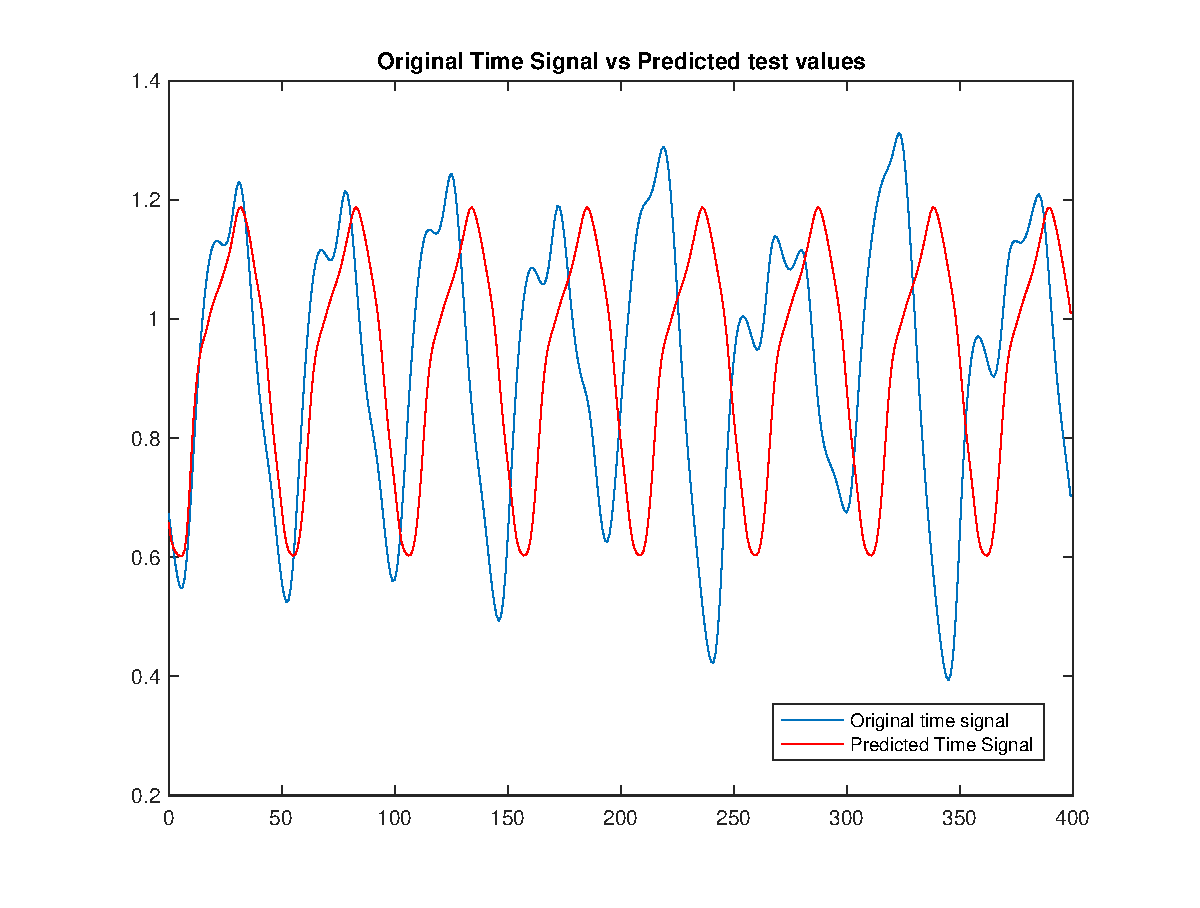
\includegraphics[clip,width=\columnwidth]{Figures/PlotTimeSeriesResult}% 
\caption{This is an example of a figure and its caption.}
\label{fig:timeseries}
\end{figure}

\begin{table}[!ht]
\renewcommand{\arraystretch}{1.50}
\caption{This is an example of a table and its caption.}
\label{tablePCA}
\centering
\begin{tabular}{| c | c |}
\hline
\bfseries PCA & \bfseries Residual mean (in absolute values) \\
\hline\hline
Original PCA & 0.1267  \\
\hline
PCA on Centroid 1 & 0.1249\\
\hline
PCA on Centroid 2 & 0.1214  \\
\hline
\end{tabular}
\end{table}

\newpage




% Conclusion and Discussion
\chapter{Discussion}

This is an example paragraph. As you can see, the main text uses a font size of 12 pt and a line spacing of 1.5. Neither the paragraphs nor the first lines of paragraphs should be indented.

There is no very strict page limit. Your number of pages will be strongly influenced by the size and total number of your figures and tables. It is recommended staying within 30-50 pages. Do not try to fill as many pages as you can. Longer theses are not necessarily of higher quality and of more non-redundant content than shorter theses. Certainly, a master thesis of 15 pages is too short, and a master thesis of 100 pages is too long.

\section{Discussion}

\section{Conclusions}


\newpage




\listoffigures
\newpage
\listoftables

% appendices come here
\bibliographystyle{naturemag}
\bibliography{bibliography}

\appendix
\chapter{Issues} %Appendix A
This section describes different issues presented and addressed during this work
	\section{Transcription issues}
		\subsection{Transcription of the missing files from Op.20}
    \begin{itemize}
    \item Op.20 No.4 - I: mm.127
		Replacing E in the first beat of the second violin, for E\#
    \end{itemize}
    \subsection{Corrections over the Altmann Edition}
    \begin{itemize}
    \item Op.20 No.2 - I: mm.29
    In the Altmann edition, the bass goes to E flat after a Dominant Seventh chord, however, in other editions it moves to the tonic, it makes more sense to the harmonic context to move towards the tonic, therefore, ignoring the spelling of the Altmann Edition for this measure and considering the bass as heading to the tonic in the third beat of the measure.
    \end{itemize}
		\subsection{Corrections over previous KernScores corpus}
    \begin{itemize}
    \item Op.20 No.4 - I: mm.124
    Changing the spelling of the viola from F natural to E sharp as it explains better a dominant seventh chord, and also, it appears like that in the Altmann Edition.

    \item Op.20 No.4 - IV: mm.24
    Adding an e natural to the first violin. It matches what is written in the Altmann Edition, and it makes the harmony clearer, from a g-diminished triad to a fully diminished e natural seventh chord, which explains better the f chord in the next measure

    \item Op.20 No.4 - IV: mm.92 \& mm.94
    Correcting wrong spelling of a note in the viola

    \item Op.20 No.6 - II: mm.5
    Changing the D in the fourth beat of the measure for a B natural, which matches the Altmann Edition
    \end{itemize}
	\section{Annotation issues}
    \subsection{Corner cases}
      \begin{itemize}
        \item Op.20 No.4 - IV: mm.6 "The augmented triad on the fifth scale degree may be used as a substitute dominant, and may also be considered as bIII+, for example in C: V+ = G-B-D\#, bIII+ = Eb-G-B, and since in every key D\# = Eb, they are the same three pitches.", Theories and Practice of Harmonic Analysis. p. 35. ISBN 0-7734-9917-2.
      \end{itemize}
		\subsection{Non-expert analysis}
    Most of the analyses were done by me, I am not an expert.
		\subsection{Fugues are too contrapunctual}
    The fourth movements of Op.20 No.2, No.5 and No.6 are fugues, these were some of the most difficult scores to analyze manually, mainly because they are very contrapunctual.
		\subsection{Flat -VII annotated as VII}
    While annotating the scores, I marked the lowered seventh degree of the minor mode simply as VII, while it should be a lowered seventh -VII. It could affect the results.
	\section{Workflow issues}    
		\subsection{Source code coming from different sources}
    The main problem is that the source code comes from different repositories, and it is difficult in terms of reproducibility to put everything together in one place and guarantee it will work.
		\subsection{Melisma array sizes}
    There was an "error" in the melisma music analyzer. The size of static structures like arrays, have been hardcoded, in long scores like Op.20 No.3 - I, the program reached buffer overflow and crashed without completing the analysis, I fixed my version of the Melisma Music Analyzer programs to correct this, but this code is not public, as I am not aware of the license of the Melisma source code. If attempting to run the analysis in these files, the programs will crash unless this is fixed.
    \begin{itemize}
    \item Op.20 No.4 - IV
    \item Op.20 No.3 - I
    \item Op.20 No.5- I
    \end{itemize}
		\subsection{tsroot harmony2humdrum and key2humdrum}
    tsroot had a different default tempo than kern2melisma, therefore, when running the analysis over files with no explicit tempo information, the result is incorrect. I fixed this in my version of the humdrum extra tools, you can download it from my fork repository. At the moment of this publication, the fix for this has not been merged in the main project repository.
	\section{Evaluation issues}
		\subsection{Chr chords are ignored}
    I am ignoring the annotations denoted as \emph{Chr} by the automatic analysis, instead of denoting a change of harmony after encountering this tag, I am preserving the previous harmonic root. This is probably wrong and should be addressed in a future evaluation.
		\subsection{Resolution of degree in secondary functions}
    Though I described the process to resolve a subfunction, I did not write this code with my harmparser. In practice, I delegated this process to the harm2kern program that is already available in the humdrum extra tools. I did not check if the parser from harm2kern is doing this process as I described it. It might be somewhat different.
	\section{Bugfixes}
  As the result of this work, a few problems were addressed
		\subsection{tsroot --meldir and --midir args}
    The implementation of tsroot has a hardcoded default value of the meldir and midir directories, when trying to change it with console arguments, the program crashed as there was some issue in the translation of the C string. This problem was detected and now it is corrected in the latest version of humdrum extras. Special thanks to Craig Sapp who double-checked this after I posted in the humdrum forum
		\subsection{tsroot tempo correction}
    As stated previously, there is a different default tempo in the tsroot program than the kern2melisma program, this means if a file has not an explicit tempo indication, the output analysis is incorrect. This was the case for the entire dataset of Op.20, so detecting and correcting this issue was crucial for this work. This fix has not been until this point merged into the official humdrum extra repository.
\newpage


\end{document}
